\documentclass[sigconf]{acmart}

%
% defining the \BibTeX command - from Oren Patashnik's original BibTeX documentation.
\def\BibTeX{{\rm B\kern-.05em{\sc i\kern-.025em b}\kern-.08emT\kern-.1667em\lower.7ex\hbox{E}\kern-.125emX}}

\usepackage{booktabs} % For formal tables
%\usepackage{enumitem}
\usepackage{multirow}
\usepackage{url}
\usepackage{paralist}
\usepackage{epsfig}
%\usepackage{algorithmic}
\usepackage{algorithm}
\usepackage{footnote}
\usepackage{threeparttable}
\usepackage{enumerate}
\usepackage{amssymb}
\usepackage{algpseudocode}
\usepackage{color}

%\usepackage[small]{caption}

\setlength{\abovecaptionskip}{0pt}
\setlength{\belowcaptionskip}{0pt}
\setlength{\textfloatsep}{3pt plus 2pt minus 2pt}

\fancyhead{}

\newcommand{\yu}[1]{{\bf \color{red} [[Yu says ``#1'']]}}
\newcommand{\lu}[1]{{\bf \color{blue} [[Lu says ``#1'']]}}
\newcommand{\KZ}[1]{{\bf \color{blue} [[Zhu says ``#1'']]}}

\newcommand\Algphase[1]{%
	\vspace*{-.4\baselineskip}\Statex\hspace*{\dimexpr-\algorithmicindent-2pt\relax}\rule{\columnwidth}{0.4pt}%
	\Statex\hspace*{-\algorithmicindent}\textbf{#1}%
	\vspace*{-.6\baselineskip}\Statex\hspace*{\dimexpr-\algorithmicindent-2pt\relax}\rule{\columnwidth}{0.4pt}%
}

% Copyright
\setcopyright{none}
%\setcopyright{acmcopyright}
%\setcopyright{acmlicensed}
%\setcopyright{rightsretained}
%\setcopyright{usgov}
%\setcopyright{usgovmixed}
%\setcopyright{cagov}
%\setcopyright{cagovmixed}


% DOI
%\acmDOI{10.475/123_4}

% ISBN
%\acmISBN{123-4567-24-567/08/06}

%Conference
%\acmConference[WOODSTOCK'97]{ACM Woodstock conference}{July 1997}{El Paso, Texas USA}
%\acmYear{1997}
%\copyrightyear{2016}
%
%
%\acmArticle{4}
%\acmPrice{15.00}

% These commands are optional
%\acmBooktitle{Transactions of the ACM Woodstock conference}
%\editor{Jennifer B. Sartor}
%\editor{Theo D'Hondt}
%\editor{Wolfgang De Meuter}


\begin{document}
%\title{Optimal K-item Set Recommendation}
\title{Exact-K Recommendation via Maximal Clique Optimization}
%\titlenote{Produces the permission block, and
%  copyright information}
%\subtitle{Extended Abstract}
%\subtitlenote{The full version of the author's guide is available as
%  \texttt{acmart.pdf} document}


\author{Anonymous Authors}
%\authornote{Dr.~Trovato insisted his name be first.}
%\orcid{1234-5678-9012}
%\affiliation{%
%  \institution{Institute for Clarity in Documentation}
%  \streetaddress{P.O. Box 1212}
%  \city{Dublin}
%  \state{Ohio}
%  \postcode{43017-6221}
%}
%\email{trovato@corporation.com}

% The default list of authors is too long for headers.
\renewcommand{\shortauthors}{Anonymous Authors}
%\renewcommand{\shorttitle}{Exact-K Recommendation}


\begin{abstract}
%\KZ{Simplify this to 4 sentences only: problem, why interesting problem,
%your solution, and what's so good about your solution.}
This paper targets to a novel but practical recommendation problem named exact-K recommendation.
It is different from traditional top-K recommendation,
as it focuses more on (constrained) combinatorial optimization which will optimize to recommend a whole set of $K$ items called card,
rather than ranking optimization 
which assumes that ``better'' items should be put into top positions.
Thus we take the first step to give a formal problem definition,
and innovatively reduce it to Maximum Clique Optimization based on graph.
To tackle this specific combinatorial optimization problem which is NP-hard, we propose \emph{Graph Attention Networks} (GAttN) with a Multi-head Self-attention encoder and a decoder with attention mechanism. 
%\yu{The insights.}
It can end-to-end learn the joint distribution of the $K$ items and generate an optimal card rather than rank individual items by prediction scores.
Then we propose \emph{Reinforcement Learning from Demonstrations} (RLfD) which combines the advantages in behavior cloning and reinforcement learning, making it sufficient-and-efficient to train the model.
Extensive experiments on three datasets demonstrate the effectiveness of our proposed \emph{GAttN with RLfD} method, it outperforms several strong baselines with a relative improvement of 7.7\% and 4.7\% on average in Precision and Hit Ratio respectively, and achieves state-of-the-art (SOTA) performance for the exact-K recommendation problem.
\end{abstract}

%
% The code below should be generated by the tool at
% http://dl.acm.org/ccs.cfm
% Please copy and paste the code instead of the example below.
%
%\begin{CCSXML}
%<ccs2012>
% <concept>
%  <concept_id>10010520.10010553.10010562</concept_id>
%  <concept_desc>Computer systems organization~Embedded systems</concept_desc>
%  <concept_significance>500</concept_significance>
% </concept>
% <concept>
%  <concept_id>10010520.10010575.10010755</concept_id>
%  <concept_desc>Computer systems organization~Redundancy</concept_desc>
%  <concept_significance>300</concept_significance>
% </concept>
% <concept>
%  <concept_id>10010520.10010553.10010554</concept_id>
%  <concept_desc>Computer systems organization~Robotics</concept_desc>
%  <concept_significance>100</concept_significance>
% </concept>
% <concept>
%  <concept_id>10003033.10003083.10003095</concept_id>
%  <concept_desc>Networks~Network reliability</concept_desc>
%  <concept_significance>100</concept_significance>
% </concept>
%</ccs2012>
%\end{CCSXML}

%\ccsdesc[500]{Computer systems organization~Embedded systems}
%\ccsdesc[300]{Computer systems organization~Redundancy}
%\ccsdesc{Computer systems organization~Robotics}
%\ccsdesc[100]{Networks~Network reliability}


%\keywords{ACM proceedings, \LaTeX, text tagging}

\maketitle

\section{Introduction}

Protein$-$protein interactions (PPIs) are of central importance for the majority of biological functions, such as signal transduction, metabolic pathways, molecular dynamics, and protein networks\cite{Hoffmann.Krallinger.ea:2005}, for they serve as the most fundamental building blocks of the entire interacademic systems of any organisms. Collecting data on pairwise interaction relationships is essential for multiple purpose, including identification of modules with certain functionality\cite{Spirin.Mirny.03}, mapping diseases to dominated genes\cite{Ideker.Sharan.08}, and after all, understanding wholistic metabolic/genetic networks from a system biology perspective.

A lot of databases have been built to store protein and genetic interactions from major model organism species and are available in various standardized formats, such as MINT\cite{Zanzoni.Montecchi-Palazzi.ea:2002}, BIND\cite{Bader.ea:2003}, BIOGRID\cite{DBLP:journals/nar/StarkBRBBT06}, etc. Among those mainstream databases, the data largely rely on voluntary reports by scientists or researchers, besides, comprehensive curation efforts become indispensable for the sake of accuracy. However, the amount of biology-related literatures with respect to protein interactions grows explosively and thus make it either impossible or impractical to manually detect PPI information anymore.

Considering huge amount of PPI information with great wealth hidden in published papers, in recent years, numerous mining techniques have been proposed that aim to extract PPI information automatically from free text, especially machine learning, information retrieval, and natural language processing\cite{DBLP:journals/bib/WinnenburgWPDS08}.These approaches can be roughly categorized into three classes: co$-$occurrence, rule$-$based, and machine learning. 

Co$-$occurrence is the approach with most simplicity and naivete. Just as its name implies, this method intends to find out pairs of proteins that co-occur in the same context. The scope of "same context" ranges from phrase, sentence, paragraph to whole abstract, even document. The underlying assumption is that whenever two proteins are mentioned together by authors, chances are high that there is some kind of relationship between them. However, however, in-context closeness even semantic relation does not necessarily represent actual biological interaction. As a consequence, a large fraction of candidate pairs are mismatched inevitably, causing a high recall but low precision.

The second approach is rule-based extraction, in other words, pattern matching. There are many types of rules, most of them concern natural language processing (NLP). One way is to specify hand-crafted regular expressions before hand, which mostly lean on language usage preference. Besides, by using full or partial (shallow) parsing strategies, more information would be acquired, such as part-of-speech taggers, local dependencies between syntactic components, context-free grammar\cite{DBLP:journals/bioinformatics/TemkinG03}, and full sentence structure. Compared to co$-$occurrence, rule-based approach enjoy better precision but much lower recall. In addition, since the rules are usually derived from training data, that is to say, the improper choice of training data would be significantly lethal, therefore quality of extraction is invariably instable and may not applicable to other data.

The third and most commonly used approach use machine learning techniques, in this case, the task to extract protein$-$protein interactions turns out to be a binary classification problem. Each protein pairs are represented along with a set of features, which is associated with their context, then a well$-$defined classifier gives the answer whether the candidate protein pairs is classified to be qualified PPI. (TO BE FURTHER FILLED!!!)

In this paper, we introduce a general bootstrapping framework for Protein$-$protein interaction extraction from natural text.Our method differs from most of the previous works in three aspects:

(1)The extraction process is driven by only tiny fraction of training data, which are regarded as seed data. In each round, it would derive reliable patterns automatically from seed data, then extract more positive PPI pairs consequently, what's more, the seed data would be augmented by the newly extracted results with high confidence.

(2)multiple graph kernel. 

(3)various evaluation.




\section{Related Work}
This section surveys previous works on question generation and tree encoding
respectively.

Text question generation has attracted the attention 
after the work of ~\citeauthor{du2017learning}~\shortcite{du2017learning}, who uses deep seq2seq model 
to generate questions from a raw text paragraph. 
Before that, text question generation relied heavily on hand-craft 
question patterns~\cite{HeilmanS10,LabutovBV15,MostowC09} which is time and 
labor consuming. 

However, this pure seq2seq model is not focused and 
has no control over part in the paragraph to generate question. 
~\citeauthor{zhou2017neural}~\shortcite{zhou2017neural} proposed to encode 
key phrase information using binary indicators to generate 
key-aware questions and they assumes the answer to be key phrase. 
Considering key phrase (answer) is unavailable in reality, 
~\citeauthor{SubramanianWYT17}~\shortcite{SubramanianWYT17} applied 
a two-stage approach. First, key phrases are extracted by 
pointer network~\cite{ptrnet}. Second, 
key phrases are encoded in the same way as 
Zhou et al. With the intuition that questions could be asked in many ways, 
~\citeauthor{Yao2018vae}~\shortcite{Yao2018vae} used conditional-VAE to 
increase the diversity of questions. More recently, models with 
auxiliary feature information~\cite{HarrisonW18} helped improve 
the question quality. Structure question generation aims at 
converting structured data such as triples in knowledge graph to questions. 
~\citeauthor{SerbanGGACCB16}~\shortcite{SerbanGGACCB16} proposed a model to generate factoid questions from knowledge base triples.  None of the above work
considered using parse tree structures to aid question generation process,
which is the focus of this paper.

Sequential RNN model takes sentence as a sequence of words, 
ignoring the syntactic information. In order to utilize
such syntactic information with sequential information, 
~\citeauthor{tai2015improved}~\shortcite{tai2015improved} proposed Tree-LSTM to 
encode the binary parse tree recursively in a bottom-up fashion to 
classify sentiment. In text generation task, 
\citeauthor{eriguchi2016tree}~\shortcite{eriguchi2016tree} 
proposed a tree-to-sequence model with attention mechanism to do 
machine translation and 
~\citeauthor{liang2018automatic}~\shortcite{liang2018automatic} proposed a 
tree-to-sequence model which could handle arbitrary trees, 
to do code comment generation. Our work is inspired by these previous
attempts and we are first to adapt structure encoded neural models to
textual question generations.
\section{Problem Definition}
\label{sec:problem}

In this section we formally define the problem of short title extraction.
A char is a single Chinese or English character.
A segmented word (or term) $x$ is a sequence of several chars such as 
``Nike'' or ``牛仔裤''(jean).
A product title, denoted as $X$, is a sequence of words $\{x_1, x_2, ..., x_n\}$.
Let $Y$ be a sequence of labels $\{y_1, y_2, ..., y_n\}$ over $X$, where $y_i \in \{0, 1\}$.
The corresponding short title is a subsequence of $X$, denoted as $S = \{x_i\}$, 
where $y_i = 1$ and $|S| \le n$.

%we are interesting in obtaining a short title which can represent the most important information about the product.

We regard short title extraction task as a sequence classification problem.
Each word is sequentially visited in the original product title order
and a binary decision is made.
We do this by scoring each word $x_i$ within $X$ and predicting a label $y_i \in \{0, 1\}$, 
indicating whether the word should or should not be included in the short title $S$.
As we apply supervised training, the objective is to maximize the likelihood of all word labels
$Y=\{y_1,y_2,...,y_n\}$, given the input product title $X$ and model parameters $\theta$:
\begin{equation}
\label{eqn:problem}
\log{p(Y|X,\theta)}=\sum_{i=1}^{n}{\log{p(y_i|X,\theta)}}.
\end{equation}

%Our problem is different from Sequece Labelling problem, as ...

%In a more restrictive scenario, the number of words $m$ in the short title is strictly limited, where $m$ is some fixed number and $m \le \sum_{i=1}^{n} len(x_i)$. $len(x_i)$ is the number of words (chars) in term $x_i$.


\section{Approach}
\label{sec:approach}
In this section, we first introduce the general framework of ChatMatch, which is modeled as
a sport tournament, then discuss some possible scoring functions that can be used by
the virtual judges in these competitions.

%Our whole evaluation framework consists of competition and scoring at three different levels. 
%The game level is at the bottom 
%and is played between two players. 
%Then comes the match level.
%To ensure the fairness of the game, 
%two games will be played between every two robots, 
%with each side starting a conversation.
%The result of two games determines the outcome of a match. 
%The tournament level is at the top
% and is composed of matches among different pairs of players. 

\subsection{Competition Protocol}
\label{sec:competition}
The competition takes place, from top to bottom, at tournament, match and
game levels.

\subsection*{Tournament Rules}
%\KZ{Give an overview of the how the tournament is run.}
We adopt a double round-robin 
sports tournament, where all bots participating in the competition 
converse directly with each other twice.
This is better than a knock-out system because it assesses a bot's ability to
deal with both strong and weak bots.
%For example, whether with weaker bots will induce them to make more mistakes or  how stronger bots will motivate their performance.
If we have $n$ chatbots players in our tournament, 
there will be $n\times (n-1) $ games in total.

\subsection*{Match Rules}
%\KZ{Talk about how the matches are administered. Just the procedure only.}
There are two chatbots competing in a single match. 
Each match consists of two games,
 started by a different bot. 
If we have $n$ bots in our tournaments, there 
will be ${n \choose 2}$ matches in total. 

\subsection*{Game Rules}
%\KZ{The procedure of the game. How each game is started and stopped.}
Each game is started by a player whose first utterance is provided by 
the system. The choice of the first utterance can be different 
depending on the domain of the bots and the ability we want to 
rank about the bots. For example, if we want to test 
the ability on movies, we can set a movie-related 
first utterance. 

During a game, there might be different ways to 
end the conversation. We can set a fixed number of exchanges 
or a terminating condition such as whether a bot makes a fatal error
or whether a certain score is reached.

\begin{table*}[th]
\centering
\scriptsize
\begin{tabular}{c|l|l}
%\hline
\toprule
\textbf{Dimension} & \textbf{Definition} &\textbf{Approach} \\ \midrule
Fluency  & Responses are fluent and natural.& Sentence perplexity. \\
Knowledge & Responses indicate the bot has the knowledge. & The number of times the bot expresses its ignorance to a question.\\
Proactivity & Responses actively proceed the conversation.&The number of times the bot raises a question. \\
Specificity & Responses are not generic.&The average of Distinct-1 and Distinct-2 \citep{li2015diversity}.\\
Diversity &Responses which are diverse and non-repetitive. &Repetition detection following the function in \algoref{algo:rep}. \\
Consistency &Responses do not contradict chat history. &Detect inconsistent questions following the function in \algoref{algo:inconsist}\\
Relevance & Responses are related to current context.& Ability to catch the relevant concept in chat history defined in \algoref{algo:bonus}. \\
\bottomrule
\end{tabular}
\caption{Seven evaluation dimensions.}
\label{tab:methods}
\end{table*}


\subsection{Scoring}
\label{sec:scoring}
\subsection*{Game-level Scoring}
%\KZ{Define a few functions: one to catch repeating, one to chat contradiction and one to catch long term memory.}

%Here we define the rules for recording points in one game between two bots. 
Inspired by \citet{finch2020towards}, 
we score each turn based on seven aspects of rules 
concerning \textit{consistency}, \textit{fluency}, \textit{knowledge}, \textit{specificity}, 
\textit{diversity}, \textit{relevance} and \textit{proactivity}. 
%As these seven metrics present a high level of 
%overlap among all distinct evaluation metrics used 
%during different process of human evaluation,
%we believe the combination of these seven distinct dimensions will be reliable. 
Finally, we sum up the scores for each bot for all the turns.
\tabref{tab:methods} documents the definition of these dimensions, which can all be scored
automatically.

%After finishing the calculation of the bonus and penalty scores for each turn, we obtain the scores of the two bots in a game with weighted sum according to \eqnref{eq:sum-up}

%\begin{equation}
%S(bot) = \sum_t - c\times C(t)  - r \times R(t) + b \times B(t)
%\label{eq:sum-up}
%\end{equation}
%$S$ denotes the total score gained by a bot for a game.
\begin{figure}[th]
        \centering
        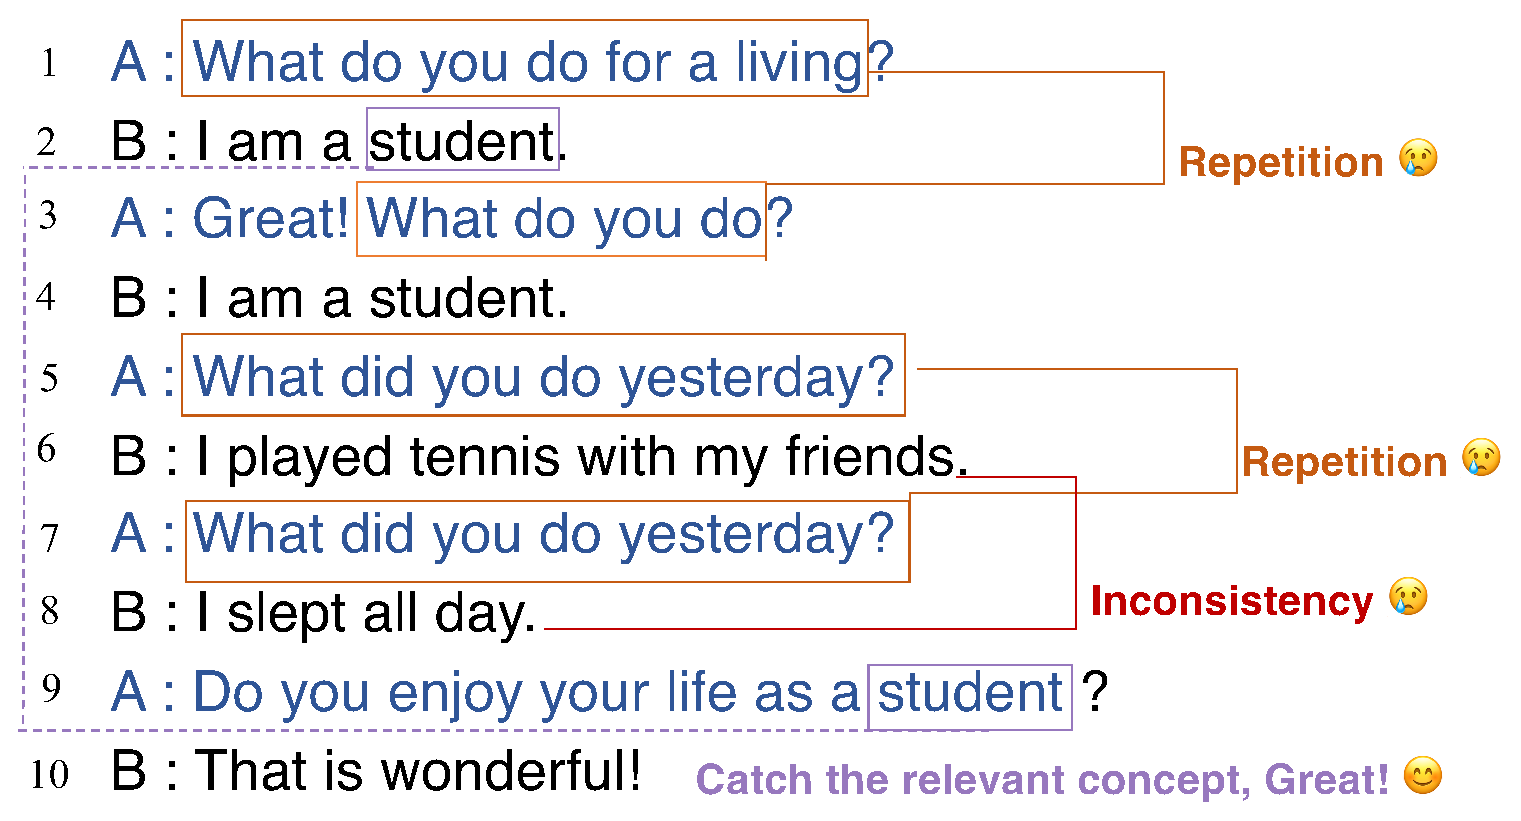
\includegraphics[width=0.95\columnwidth]{example2.eps}
        \caption{A chat snippet between two bots.}
        \label{fig:example}
\end{figure}

Fluency, Knowledge, Proactivity and Specificity are scored for each turn separately
and aggregated at the end of the conversation.
Detection for diversity, consistency and relevance are more involved and are explained
using \figref{fig:example}. 

As for diversity, at each turn $t$, we first check if there exists any repetitive question.  
We can easily find turn 3 and turn 7 repeated turn 1 and turn 5 
respectively. They will then be penalized one point for repetition. 
Repetition is not penalized if the previous turn is already 
marked as a repetitive question. For example, in \figref{fig:example}, 
although turn 4 is considered a repetition of turn 2,  
we are not going to penalize it as turn 3 is a repetitive question. 

The detection of inconsistency is always triggered after the detection of repeated questions. 
If the answers to the same questions are different, we will penalize the current turn, 
such as turn 8 in \figref{fig:example}.

We decide a repetition or an inconsistency by calculating the similarity of the two turns. 
We use a similarity function to complete the calculations, which we will 
discuss in \secref{sec:experiment}. The actual diversity and consistency scores
are the negation from the amount of repetition and inconsistency.

Relevance is assessed as a bonus to reward
a bot if it is able to memorize the important relevant concepts that have shown up 
before in the conversation. We sort the concepts that have shown up in 
chat history by their IDF scores. For example, in turn 9, $A$ 
mentions the concept word ``student'' presented by $B$ in turn 2. With this
turn, $A$ will win a bonus point.


The algorithms and notations for computing diviersty, consistency and relevance are included
in \tabref{tab:functions}, \algoref{algo:rep}, \algoref{algo:inconsist}, and \algoref{algo:bonus}. 

\begin{table}[th]
\centering
\small
\begin{tabular}{c|l}
%\hline
\toprule
\textbf{Notation} & \textbf{Description} \\ \midrule
$t$ & Current turn \\
$H(t)$  &  a list of history turns prior to $t$ \\
$Sim(x,y)$ & similarity between two turns $x$ and $y$ \\
$\sigma_r$ & Threshold for detecting repetition \\
$\sigma_c$ & Threshold for detecting consistency \\
$r$ & Weight for repetition \\
$c$ & Weight for inconsistency \\
$b$ & Weight for bonus \\
$d$ & Min distance between consecutive mentions \\
IDF list & List of lemma in chatlog sorted by IDF\\
$p$ & Percentage of important lemmas in IDF list\\
$R(t)$ &  Repetition penalty for turn $t$ \\
$C(t)$ &  Inconsistency penalty for turn $t$ \\ 
$B(t)$ &  Memory bonus for turn $t$ \\
$Rep(t)$ & A list of repeated turns for turn $t$ \\  
\bottomrule
\end{tabular}
\caption{
Functions and variables in algorithms.}
\label{tab:functions}
\end{table}

\begin{algorithm}[th]
\small
\caption{Scoring for Diversity}
\label{algo:rep}
\hspace*{0.02in} {\bf Input:}
 $t$, $H$, $Sim$, $\sigma_{r}$
; \hspace*{0.02in} {\bf Output: } 
 $R$;
\begin{algorithmic}[1]
\State //Starting to detect repetition
\For {$u$ in $H(t)$}
	\If {$Sim(t,u) \geq \sigma_{r}$}
		\State Add $u$ to $Rep(t)$
	\EndIf
\EndFor
    \If{$len(Rep(t))\geq 0$}
        \If{$t$ is a question and We can find a question in $Rep(t)$}
        \State $ R(t) \leftarrow  R(t) + 1$ 
        \Else
        \If {the previous turn of $t$ is not a repetitive question}
        \State $R(t)) \leftarrow R(t) + 1$ 
        \EndIf
        \EndIf
    \EndIf
\end{algorithmic}
\end{algorithm}


\begin{algorithm}[th]
\small
\caption{Scoring for Consistency}
\label{algo:inconsist}
\hspace*{0.02in} {\bf Input:}
$t$, $H$, $Sim$, $\sigma_{c}$
; \hspace*{0.02in} {\bf Output:  } 
 $C$;
\begin{algorithmic}[1]
\State // Inconsistency detection
 \If {previous turn of $p$ is a repetitive question} 
   \If{ the response $res$ to the question repeated by turn $p$ contradicts turn $i$ with $Sim(t, res) \leq \sigma_{c}$ }
    \State $C(t) \leftarrow C(t) + 1$
   \EndIf
  \EndIf
\end{algorithmic}
\end{algorithm}

\begin{algorithm}[th]
\small
\caption{Scoring for Relevance}
\label{algo:bonus}
\hspace*{0.02in} {\bf Input:}
$t$, $p$, $d$
; \hspace*{0.02in} {\bf Output:  } 
$B$;
\begin{algorithmic}[1]
\State // Assessing the ability of catching relevant concepts\\
$B(t) \leftarrow 0$
\For {all tokens $tk$ in current turn $t$}
 \If {$t$ - previous occurrence turn of $tk > d$ and $tk$ in the top $p\%$ of the IDF list of all tokens in the dialogue} 
   \State $B(t) \leftarrow 1$
  \EndIf
 \EndFor
\end{algorithmic}
\end{algorithm}

At the end of each game, each bot gets seven scores, one for each dimension.  
After pairwise comparison on individual dimension, a bot gains one point for win and zero point for a tie or lose.
The final score of each bot is determined by the sum of their individual scores.
%\KZ{Are these scores positive or negative? Comparable between bots?}

\subsubsection*{Match-level Scoring}
%\KZ{Use an equation to compute the final scores?}
One match which consists of two games, each started with a different bot, 
decides winning or losing between two bots.
For match-level scoring, we mimic the scoring rules of soccer tournament. 
For each match, $W$ points for the winner,  
$T$ points for a tie and 
$L$ points for the loser.
The value of $W$, $T$ and $L$ will be discussed in \secref{sec:ablation}. 

%\KZ{At the match level, we need to consider different starting context for the bots? I think we should present a few options for the reader and say that we are limited to these.}

\subsubsection*{Tournament-level Scoring}
%\KZ{Use an equation to compute the final scores?}
We count the points by simply summing up their scores gained in every match. Currently, several bots with the same final rank are tolerated. For future study, it's possible to mimic more detailed rules presented in sports match such as determine their ranking based on their win-loss relationship in the match between them.  
If they are still tied, we could propose an “overtime” for these two bots, one human judge may observe their performance and then make the decision of the game.

\section{EXPERIMENT EVALUATION}
In this section, we conduct extensive experiments to evaluate the effect of our proposed solution to derive causality knowledge. All the experiments are implemented in Python and run on a Intel Xeon 32 CPU(2.60GHz) with 173GB memory.


\subsection{Dataset}
The dataset crawled from financial news website \footnote{ \url { http://finance.sina.com.cn }} contains \textbf{4 991 000} articles, and there are \textbf{111 330 205} sentences. The number of unique sentences is \textbf{75 572 053}, occupied  \textbf{67.88\%} of the total sentences. The number of sentence with casual cue words is \textbf{7 147 141}, occupied \textbf{9.46\%}.

\textbf{Causal Pattern statistic.} The elaborate casual patterns can be grouped into 6 groups of templates, each containing pattern in one group  has the same meaning but different words. The matched sentences distribution over these groups of patterns is shown in Fig.\ref{tab3}. from which, we can find the first three take most proportion of the whole sentences. and we will use these three kind of sentence to carry on later experiments.
\begin{table*}[t]
	\caption{Number of sentences extracted by causal patterns}
	\begin{center}
		\begin{tabular}{|c|c|c|c|}
			\hline
			\textbf{Pattern template}& \textbf{Pattern}& \textbf{Number}& \textbf{Rate}\\
			\hline
			A->B&因为 A,B&2000242&0.4831573605311576\\
			\hline
			A->B&A,所以 B&1530311&0.4831573605311576\\
			\hline
			A->B&因为 A, 所以B&2000242&0.3696457846359572\\
			\hline
			$A_1,A_2->B$&因为 $A_1$, 且 $A_2$, 所以 B&22356&0.005400079566389746\\
			\hline
			$A->B_1,B_2$&因为 A,所以 $B_1$ 且 $B_2$&10178&0.002458490330413081\\
			\hline
			$A_1,A_2->B_1,B_2$&因为 $A_1$, 且 $A_2$,所以 $B_1$  且 $B_2$&1&2.415494527817922e-07\\
			\hline
		\end{tabular}
		\label{tab3}
	\end{center}
\end{table*}	


\textbf{Our newly built Knowledge Base.}
TODO: explaination
\begin{table}[t]
	\caption{Knowledge Base}
	\begin{center}
		\begin{tabular}{|c|c|}
			\hline
			\textbf{Name}&\textbf{Number}\\
			\hline
			IsA pairs (Taxonomy)&515163\\
			\hline
			Concepts (Taxonomy)&81082\\
			\hline
			instances (Taxonomy)&158693\\
			\hline
			Common Sense Pairs&7316977\\
			\hline
		\end{tabular}
		\label{tab3}
	\end{center}
\end{table}	

\textbf{Rule.}
some numbers of the rule instances, candidate instances and final rules are show in \ref{tab3}.
\begin{table}[t]
	\caption{Rule number}
	\begin{center}
		\begin{tabular}{|c|c|}
			\hline
			\textbf{Name}&\textbf{Number}\\
			\hline
			Rule Instances&??\\
			\hline
			Candidate Rules&??\\
			\hline
			Relation Number&??\\
			\hline
		\end{tabular}
		\label{tab3}
	\end{center}
\end{table}	

\subsection{Case Study}

Here we show some rules derived, some are good\ref{fig:good_rule_case}, some are bad \ref{fig:bad_rule_case}. Also, We would do some error analysis.
\subsubsection{Good Cases}
\begin{figure}[htbp]
	\centerline{\includegraphics[width=0.9\columnwidth]{figures/good_rule_case}}
	\caption{Good Cases.}
	\label{fig:good_rule_case}
\end{figure}	
	TODO: explanation   
	
\subsubsection{Bad Cases}
\begin{figure}[htbp]
	\centerline{\includegraphics[width=0.9\columnwidth]{figures/bad_rule_case}}
	\caption{Bad Cases.}
	\label{fig:bad_rule_case}

\end{figure}
	TODO: explanation why they are bad
	




\subsection{Rule instantiation}
Rule instantiation also called Rule deduction is shown in \ref{fig:instantiation}
\begin{figure}[htbp]
	\centerline{\includegraphics[width=0.9\columnwidth]{figures/instantiation}}
	\caption{Rule Instantiation .}
	\label{fig:instantiation}
\end{figure}

%\textit{Question Answer}
%\textit{Make decision}







\section{Conclusion}
We implement a novel sequence-based dependency parsing
framework which takes advantage of high order features 
in parsing history. 
%We can also adapt beam search to this framework so as to
%relax the strictly greedy nature. Vine pruning\cite{rush2012vine} could
%be incorporated to speed up the parsing.
More importantly, we discovered that the parsing accuracy is very sensitive to
the quality of parsing sequence. Future work can be focused on
developing better sequence predictors that outperform Malt action classifier.
Furthermore, we use two sets of features for sequence predictor and
head mapper right now. A unified set of features between these two components
are worth exploring.
%Besides, better sequence predicting method and unified feature
%representation of two components are worth exploring.
%
%Though we currently get a not bad result,
%the sequence predictor still needs more exploration.
%According to our experiment, slightly changes
%on the sequence can lead to a fatal decline on accuracy. Ensuring the match degree of training sequence and testing
%sequence demands a high quality of sequence predictor.
%
%Further, the features in our current implementation are not expanded and well tuned yet  and we are free to define high order features to make use of parsing history. Our framework is flexible to merge other technics to enhance the performance. Introducing beam could make up for our greedy decoder and improve our accuracy. Vine pruning\cite{rush2012vine} could speed up parsing process. Besides, better sequence predicting method and unified feature representation of two components are worth exploring.


\bibliographystyle{ACM-Reference-Format}
\bibliography{ref}

\newpage
\appendix
\section{Naive Node-Weight Estimation Method}
\begin{algorithm}
	\caption{Naive Node-Weight Estimation Method.}       
	\label{alg:naive} 
	\begin{algorithmic}[1]
		\Require Given user $u$ and candidate items set $S$, construct graph $\mathbb{G}(\mathcal{N},\mathcal{E})$ defined in paragraph 2 of Sec. \ref{sec:problem_definition}.
		\State Estimate weight $w_i$ of each node $n_i\in \mathcal{N}$ in graph based on CTR of corresponding item $s_i\in S$.
		\State Initial result card $A=\emptyset$.
		\For {\emph{t = 1 to K}}
		\State Select node $a_t$ with the largest weight in $\mathcal{N}$ and add to $A$.
		\State Remove $a_t$ and nodes in $\mathcal{N}$ which are not adjacent to $a_t$.
		\EndFor\\
		\Return result card $A$.
	\end{algorithmic}
\end{algorithm}

\section{Reinforcement Learning from Demonstrations}
\begin{algorithm}
	\caption{Reinforcement Learning from Demonstrations.}       
	\label{alg:RLfD}
	\begin{algorithmic}[1]
		\Algphase{Phase 1 - Reward Estimator Training}
		\Require reward function $P(r=1|A,u;\phi)$, dataset $P_{data}^{D}(r^*|A,u)$
		\State Optimize $\phi$ with gradient descent by loss function $\mathcal{L}_{D}(\phi)$.\\
		\Return $P(r=1|A,u;\phi^*)$
	\end{algorithmic}
	\begin{algorithmic}[1]
		\Algphase{Phase 2 - Policy Training}
		\Require optimized reward function $P(r=1|A,u;\phi^*)$, dataset $P_{data}^{S}(A^*|S,u)$, policy $P(A|S,u;\theta)$
		\State Optimize $\theta$ with gradient descent by loss function $\mathcal{L}(\theta)$.\\
		\Return $P(A|S,u;\theta^*)$
	\end{algorithmic}
\end{algorithm}

\section{Experimental Settings}
\subsection{Datasets}
%\subsubsection{Statistics}
\begin{table}[h]
	\caption{Statistics of the experimented datasets.}
	%\vspace{-10pt}
	\label{tab:dataset_statistic}
	\centering
	\scriptsize
	\begin{tabular}{c|c|c|c|c}
		\toprule
		\textbf{Dataset} & \textbf{User\#} & \textbf{Card\#} & \textbf{Item\#} & \textbf{Sample\#} \\
		\midrule
		MovieLens(K=4,N=20) & 817 & 40036 & 1630 & 40036 \\
		\midrule
		MovieLens(K=10,N=50) & 485 & 33196 & 1649 & 33198 \\
		\midrule
		Taobao(K=4,N=50) & 581055 & 310509 & 3148550  & 1116582 \\
		\bottomrule
	\end{tabular}
\end{table}
%\subsubsection{Example}
\begin{table}[h]
	\caption{Show case of the dataset.}
	%\vspace{-10pt}
	\label{tab:dataset_example}
	\centering
	\scriptsize
	\begin{threeparttable}
	\begin{tabular}{c|c|c|c|c|c}
		\toprule
		& \textbf{user} & \textbf{card} & \textbf{candidate items} & \textbf{card label} & \textbf{positive item} \\
		\midrule
		sample\#1 & 1 & 1,2,3,4 & 1,2,3,4,...,20 & 1 & 2 \\
		%\midrule
		sample\#2 & 1 & 1,4,5,6 & 1,2,3,4,...,20 & 0 & / \\
		%\midrule
		\multicolumn{6}{c}{...} \\
		\bottomrule
	\end{tabular}
	\begin{tablenotes}
		\footnotesize
		\item (We take $K=4$ and $N=20$ for example. Items and users are represented as IDs here. Card label represents whether the card is clicked or satisfied by user (labeled as 1) or not (labeled as 0). Positive item is the actually clicked item in card by user.)
	\end{tablenotes}
	\end{threeparttable}
\end{table}

\subsection{Implementation and Parameter Settings}
\label{sec:implementation}
Here we report implementation details for the three datasets\footnote{The code and datasets will be released.} (two MovieLens based datasets and one Taobao based dataset),
and our implementation is based on TensorFlow\footnote{\url{https://www.tensorflow.org/}}.
To construct the training and test sets, we perform a 4:1 random splitting as in \cite{wang2017irgan} for all the datasets.
\subsubsection{MovieLens}
\label{sec:implementation_movielens}
Notice both MovieLens(K=4,N=20) and MovieLens(K=10,N=50) share the same parameter settings.
For a fair comparison, all models are set with an embedding size of $16$ for item and user IDs,
and optimized using the mini-batch Adam \cite{kingma2014adam} with a batch size of $32$ and learning rate of $0.001$.
All models are trained for $10$ epoch.
All the trainable feed-forward parameter matrices are set with the same input and output dimension as $32\times32$ (including DeepRank, BPR, and all the RNN cells in both Listwise-GRU, Listwise-MHSA and ours). 
Specifically for our GAttN model, in decoder (in Sec. \ref{sec:decoder}) we use LSTM \cite{hochreiter1997long} cells with units number of 32 and set beam size as $3$, number of heads in encoder (in Sec. \ref{sec:encoder}) MHSA layer is $2$, and the coefficient parameter $\alpha$ in loss function (in Sec. \ref{sec:loss_combination}) is $0.5$.
Number of layers $L$ in both encoder and decoder are set as 2.
For reward estimator model (in Sec. \ref{sec:reinforce}), we set the hidden size in fully-connected layer as 128.

\subsubsection{Taobao}
\label{sec:implementation_taobao}
In this dataset, the feature vectors for user and item are statistic features with size of 40 and 52 specifically, instead of ID features.
Sample statistic features are PV (page view), IPV (item page view), GMV (cross merchandise volume), CTR (click through rate) and CVR (conversion rate) for 1 day, 7 days and 14 days, etc. 
For this dataset, we first transfer the input representation of user and item to 32 dimension, i.e we set $W_I\in \mathbb{R}^{92\times32}$ and $b_I\in \mathbb{R}^{32}$ in Sec. \ref{sec:input}.
And all the other hyper-parameters are set as the same with those on MovieLens based datasets (refer to Appx. \ref{sec:implementation_movielens}).

\end{document}
